\documentclass[tikz,10pt]{standalone}
\usetikzlibrary{positioning, calc, arrows.meta}
\DeclareMathSizes{10}{10}{5}{1}
\begin{document}
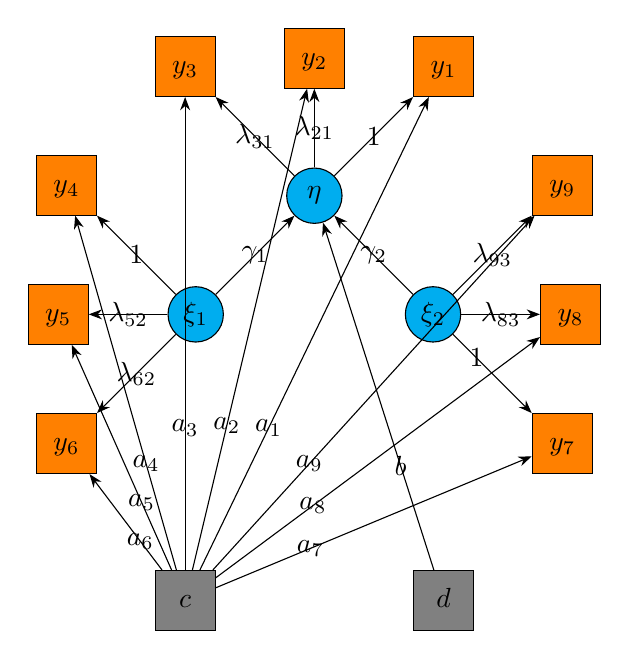
\begin{tikzpicture}
    [
        basic/.style = {draw, text centered},
        circ/.style = {basic, circle, minimum size=2em, inner sep=1.5pt, fill=cyan},
        rect/.style = {basic, text width = 1.5em, text height=1em, text depth=.5em, fill=orange},
        rectgray/.style = {basic, text width = 1.5em, text height=1em, text depth=.5em, fill=gray},
        >={Stealth[]}
    ]
    \node [circ] (base) {$\eta$};
    \node [circ, below left=of base] (xi1) {$\xi_1$};
    \node [circ, below right=of base] (xi2) {$\xi_2$}; 

    \node [rect, above right=of base] (y1) {$y_1$};
    \node [rect, above=of base] (y2) {$y_2$};
    \node [rect, above left=of base] (y3) {$y_3$};
    
    \node [rect, above left=of xi1] (y4) {$y_4$};
    \node [rect, left=of xi1] (y5) {$y_5$};
    \node [rect, below left=of xi1] (y6) {$y_6$};

    \node [rect, above right=of xi2] (y9) {$y_9$};
    \node [rect, right=of xi2] (y8) {$y_8$};
    \node [rect, below right=of xi2] (y7) {$y_7$};
    
    %\node [below right=of xi1] (tmp) {};

    \node [rectgray, below left=4.5cm and 1cm of base] (c) {$c$};
    \node [rectgray, below right = 4.5cm and 1cm of base] (d) {$d$};

    %\foreach \i/\j in {base/y1, base/y2, base/y3, xi1/y4, xi1/y5, xi1/y6, xi2/y7, xi2/y8, xi2/y9, xi1/base, xi2/base} \draw [->] (\i) -- (\j);
    \draw [->] (base) -- (y1) node[midway] {1};
    \draw [->] (base) -- (y2) node[midway] {$\lambda_{21}$};
    \draw [->] (base) -- (y3) node[midway] {$\lambda_{31}$};

    \draw [->] (xi1) -- (y4) node[midway] {1};
    \draw [->] (xi1) -- (y5) node[midway] {$\lambda_{52}$};
    \draw [->] (xi1) -- (y6) node[midway] {$\lambda_{62}$};

    \draw [->] (xi2) -- (y7) node[pos=0.3] {1};
    \draw [->] (xi2) -- (y8) node[midway] {$\lambda_{83}$};
    \draw [->] (xi2) -- (y9) node[midway] {$\lambda_{93}$};
    
    \draw [->] (xi1) -- (base) node[midway] {$\gamma_1$};
    \draw [->] (xi2) -- (base) node[midway] {$\gamma_2$};

    \foreach \i in {1, ..., 9} \draw [->] (c) -- (y\i) node[pos=0.3] {$a_\i$};

    \draw [->] (d) -- (base) node[pos=0.3] {$b$};

\end{tikzpicture}
\end{document}